\documentclass[a4paper,12pt]{article}

\usepackage[T2A]{fontenc}
\usepackage[utf8]{inputenc}
\usepackage[english,russian]{babel}

% \usepackage{minted}
\usepackage{amsmath, amsfonts, amsthm}
\usepackage{listings, listings-rust}
\usepackage{enumerate}
\usepackage{siunitx}
\usepackage{float}
\usepackage{graphicx}
\graphicspath{ {./images/} }
\usepackage{nameref}
\usepackage{hyperref}
\usepackage{tabularx}
\usepackage[top=3cm,bottom=3cm,left=2.5cm,right=2.5cm]{geometry}

\hypersetup{
	colorlinks=true,
	linkcolor=blue,
	filecolor=magenta,
	urlcolor=cyan
}
\urlstyle{same}

% \setminted{
%   frame=lines,
%   framesep=2mm,
%   baselinestretch=1.2,
%   fontsize=\footnotesize,
%   linenos
% }

% !TeX spellcheck = en_GB
% !TeX spellcheck = ru_RU

\begin{document}

\begin{titlepage}	% начало титульной страницы

	\begin{center}		% выравнивание по центру

		\large Санкт-Петербургский политехнический университет Петра Великого\\
		\large Институт компьютерных наук и технологий\\[6cm]
		% название института, затем отступ 6см

		\huge Курсовая работа\\[0.5cm] % название работы, затем отступ 0,5см
		\large Колесная платформа\\[0.1cm]
		\large по дисциплине <<Микропроцессорные системы>>\\[5cm]

	\end{center}

	\noindent\large Выполнили: \hfill \large Ферапонтов М.В.\\
	\hspace*{\fill} \large  Савчук А.А.\\
	\hspace*{\fill} \large Дорошин Д.А.\\
	\hspace*{\fill} \large Луцай П.П.\\
	\hspace*{\fill} \large Артеев Д.Д.\\
	\hspace*{\fill} \large Яровой В.Д.\\
	\noindent\large Группа: \hfill \large гр. 3530904/00104\\

	\noindent\large Проверил: \hfill \large Круглов С.К.

	\vfill % заполнить всё доступное ниже пространство

	\begin{center}
		\large Санкт-Петербург\\
		\large \the\year % вывести дату
	\end{center} % закончить выравнивание по центру

\end{titlepage} % конец титульной страницы

\vfill % заполнить всё доступное ниже пространство


\tableofcontents
\newpage

\section{Аппаратная реализация1}
\subsection{Raspberry pi 2b+}
При разработке был изпользован Raspberry Pi 2 model B+.
\begin{center}
  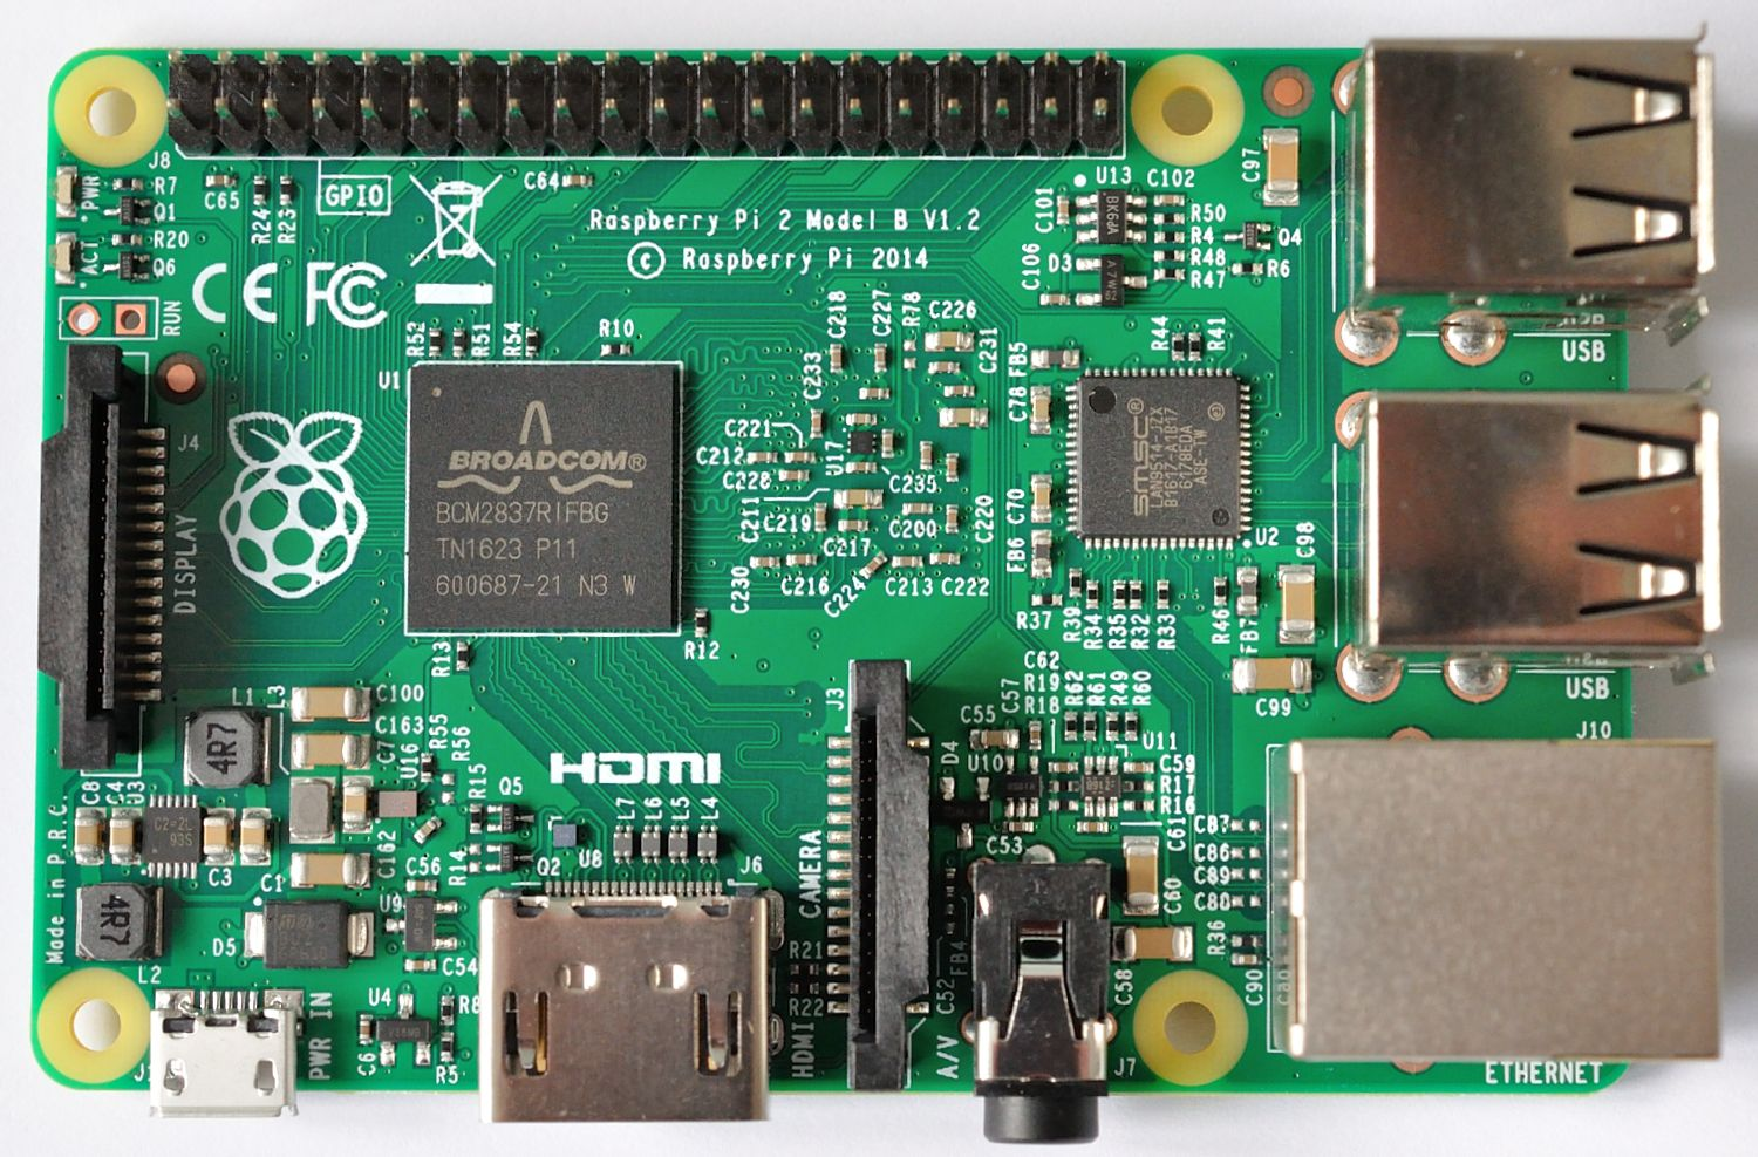
\includegraphics[width=\textwidth]{raspberry_pi2_b.pdf}
\end{center}
Характеристики:
\begin{itemize}
  \item Процессор - ARM Cortex-A7 CPU 900MHz
  \item Количество ядер - 4
  \item Оперативная память - 1Gb
\end{itemize}


\subsection{Используемые детали и модули}
Были использованы детали из набора Arduino
\begin{enumerate}
  \item Драйвер управления движения моторов L289N
  \item Колеса 4 шт.
  \item Кнопка для управления движения 4шт.
  \item Резистр 22\unit{\Omega} 4 шт
  \item Корпус
  \item Плата расширения
\end{enumerate}

Драйвер L298N используется для многофункционального управления двигателями постоянного тока.
Схема модуля, состоящая из двух H-мостов, позволяет подключать к нему один биполярный шаговый двигатель или одновременно два щёточных
двигателя постоянного тока. При этом есть возможность изменять скорость и направление вращения моторов. Управление осуществляется путём
подачи соответствующих сигналов на командные входы, выполненные в виде штыревых контактов. На рисунке показан внешний вид модуля с кратким
описанием всех его составляющих.
\begin{center}
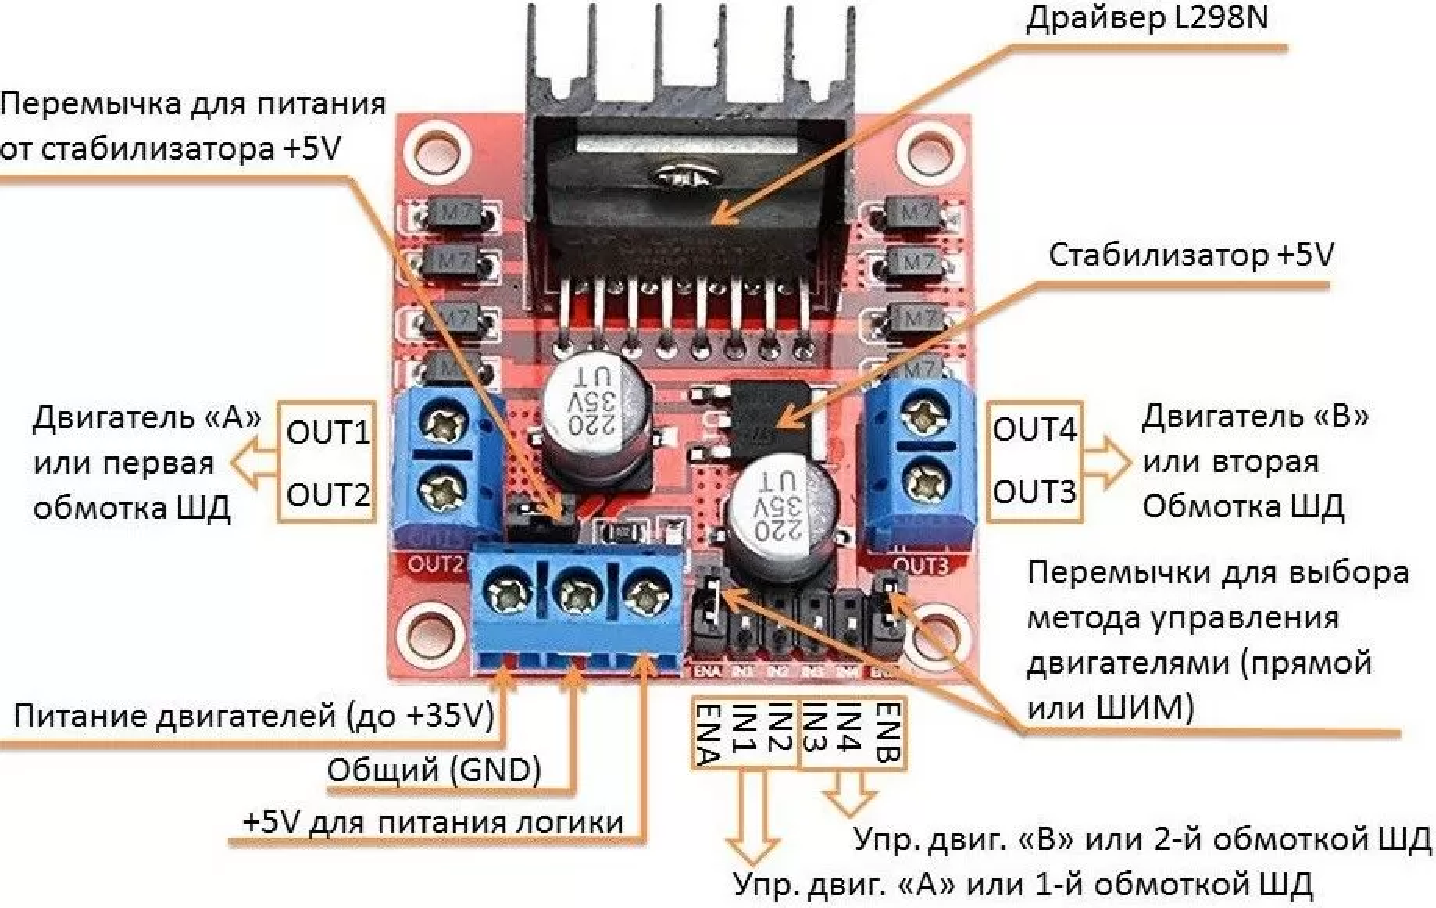
\includegraphics[scale=0.5]{l298n.pdf}
\end{center}

\subsection{Широтно-импульсная модуляция}

В драйвере L289N \textit{ENA}, \textit{ENB} –  контакты для активации/деактивации первого и второго двигателей или соответствующих обмоток ШД.
Подача логической единицы на эти контакты разрешает вращение двигателей, а логический ноль – запрещает.
Для изменения скорости вращения щёточных моторов на эти контакты подаётся ШИМ-сигнал.

\textbf{ШИМ} - метод уменьшения средней мощности, передаваемой электрическим сигналом, путем эффективного разделения его на отдельные части.
Среднее значение напряжения (и тока), подаваемого на нагрузку, регулируется быстрым включением и выключением переключателя между питанием и нагрузкой.
Чем дольше переключатель включен по сравнению с периодами выключения, тем выше общая мощность, подаваемая на нагрузку.

\begin{lstlisting}[language=Rust, style=boxed]
  pub fn set_frequency(&self, frequency: f64, duty_cycle: f64) -> Result<()>
\end{lstlisting}

\begin{itemize}
  \item frequency - частота
  \item duty cycle - скважность, задается числом с плавающей точкой в промежутке между 0.0 и 1.0.
\end{itemize}
В нашей программе изначально значение скважности установлено на 0, что означает что на двигатели будет подаваться в среднем 0\unit{\volt}. Никакого
движения не происходит. При нажатии на конпку мы подаем сигналы на левые и правые двигатели и устанавливаем скважность на 1, что означает что на двигатели
будет подаваться в среднем 5\unit{\volt}.

\begin{center}
  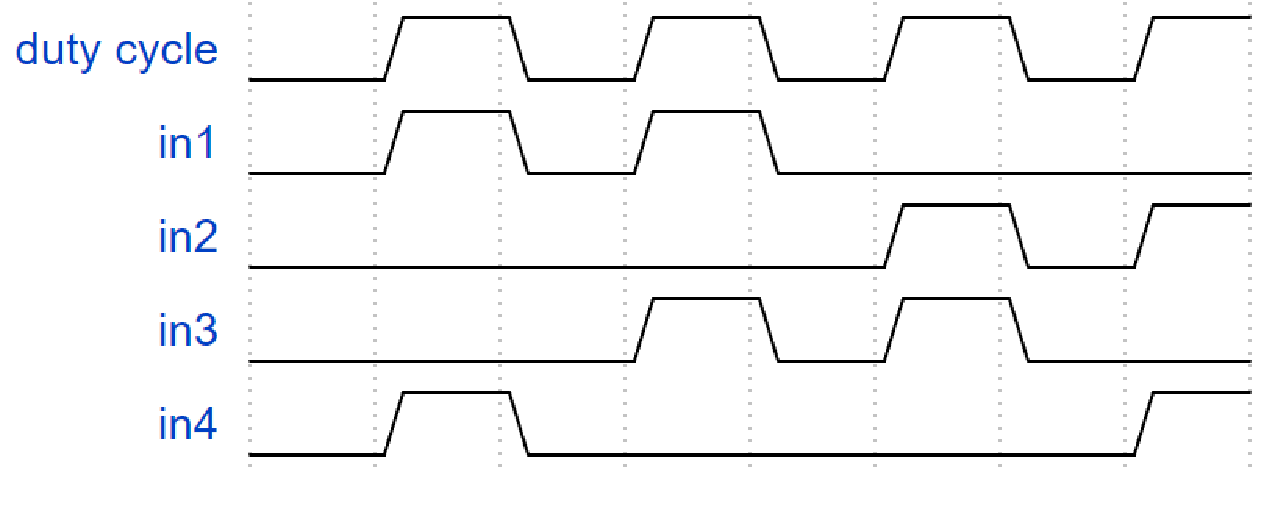
\includegraphics[width=\textwidth]{waveform.pdf}
\end{center}

\subsection{Питание}
\begin{enumerate}
  \item L289N - Логическое устройство - 5\unit{\volt}
  \item L289N - Моторы - 12\unit{\volt}
  \item Кнопка - 3.3\unit{\volt}
  \item Raspberry pi 2b+ - 5\unit{\volt}
\end{enumerate}

\section{Схемы}
\subsection{Принципиальная схема драйвера L289N}

\begin{center}
  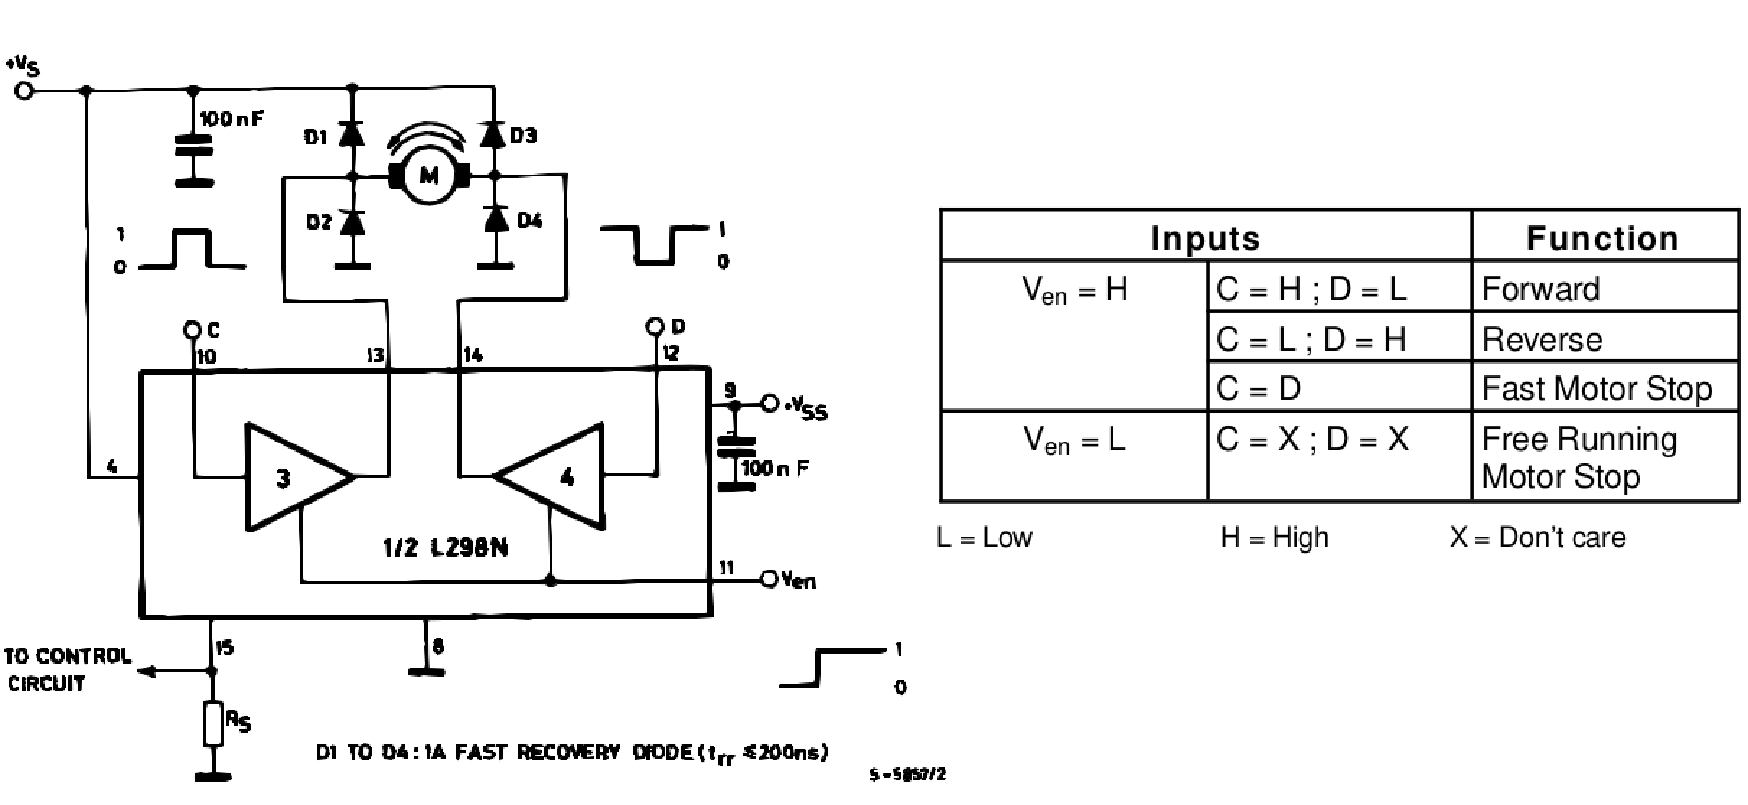
\includegraphics[scale=0.5]{dire.pdf}
\end{center}
\begin{center}
  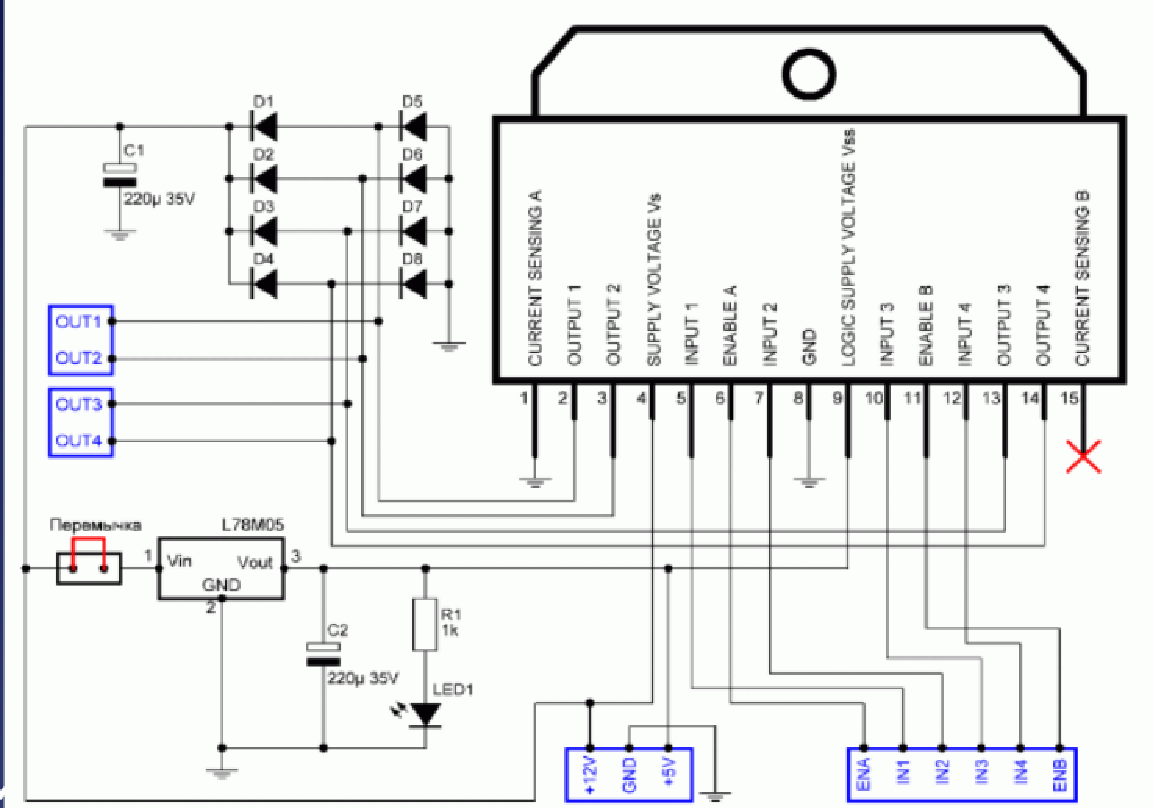
\includegraphics[scale=0.5]{bort.pdf}
\end{center}
\begin{center}
  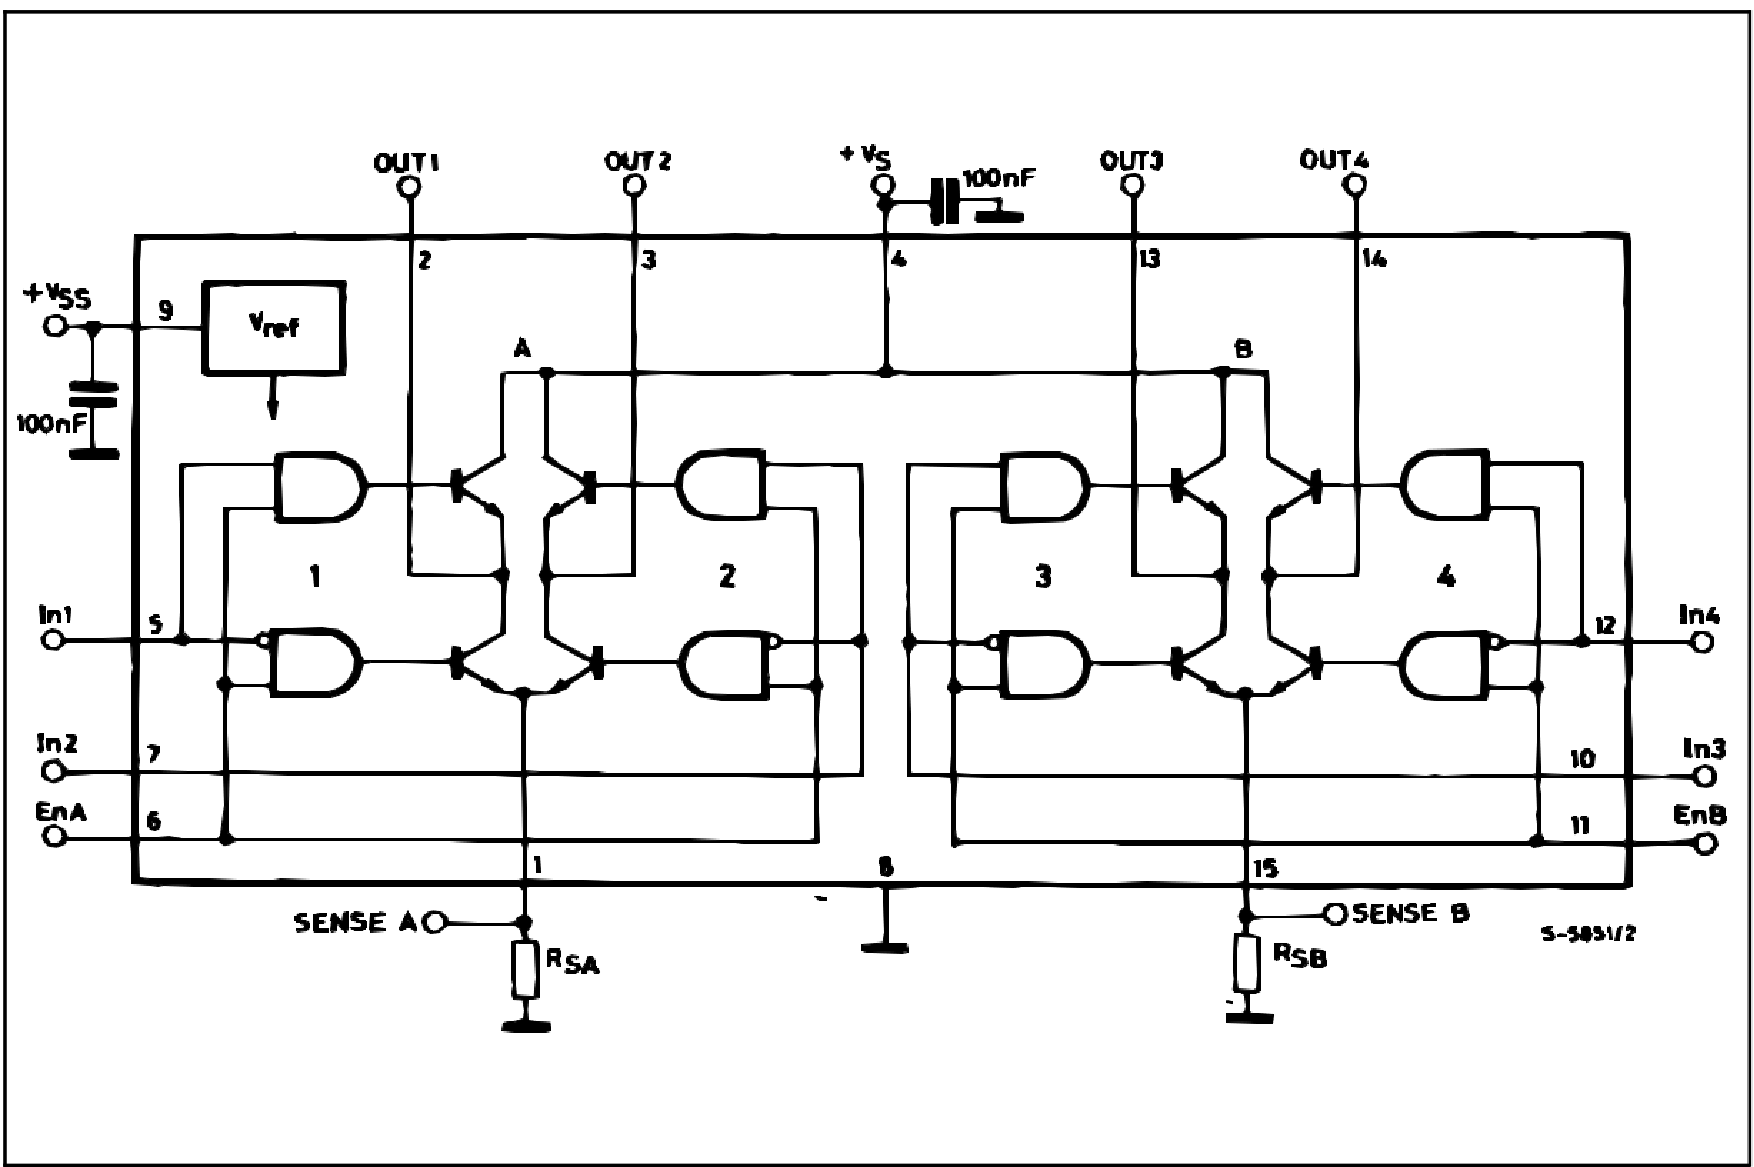
\includegraphics[scale=0.5]{chip.pdf}
\end{center}

\subsection{Принципиальная схема Raspberry Pi}
\begin{center}
  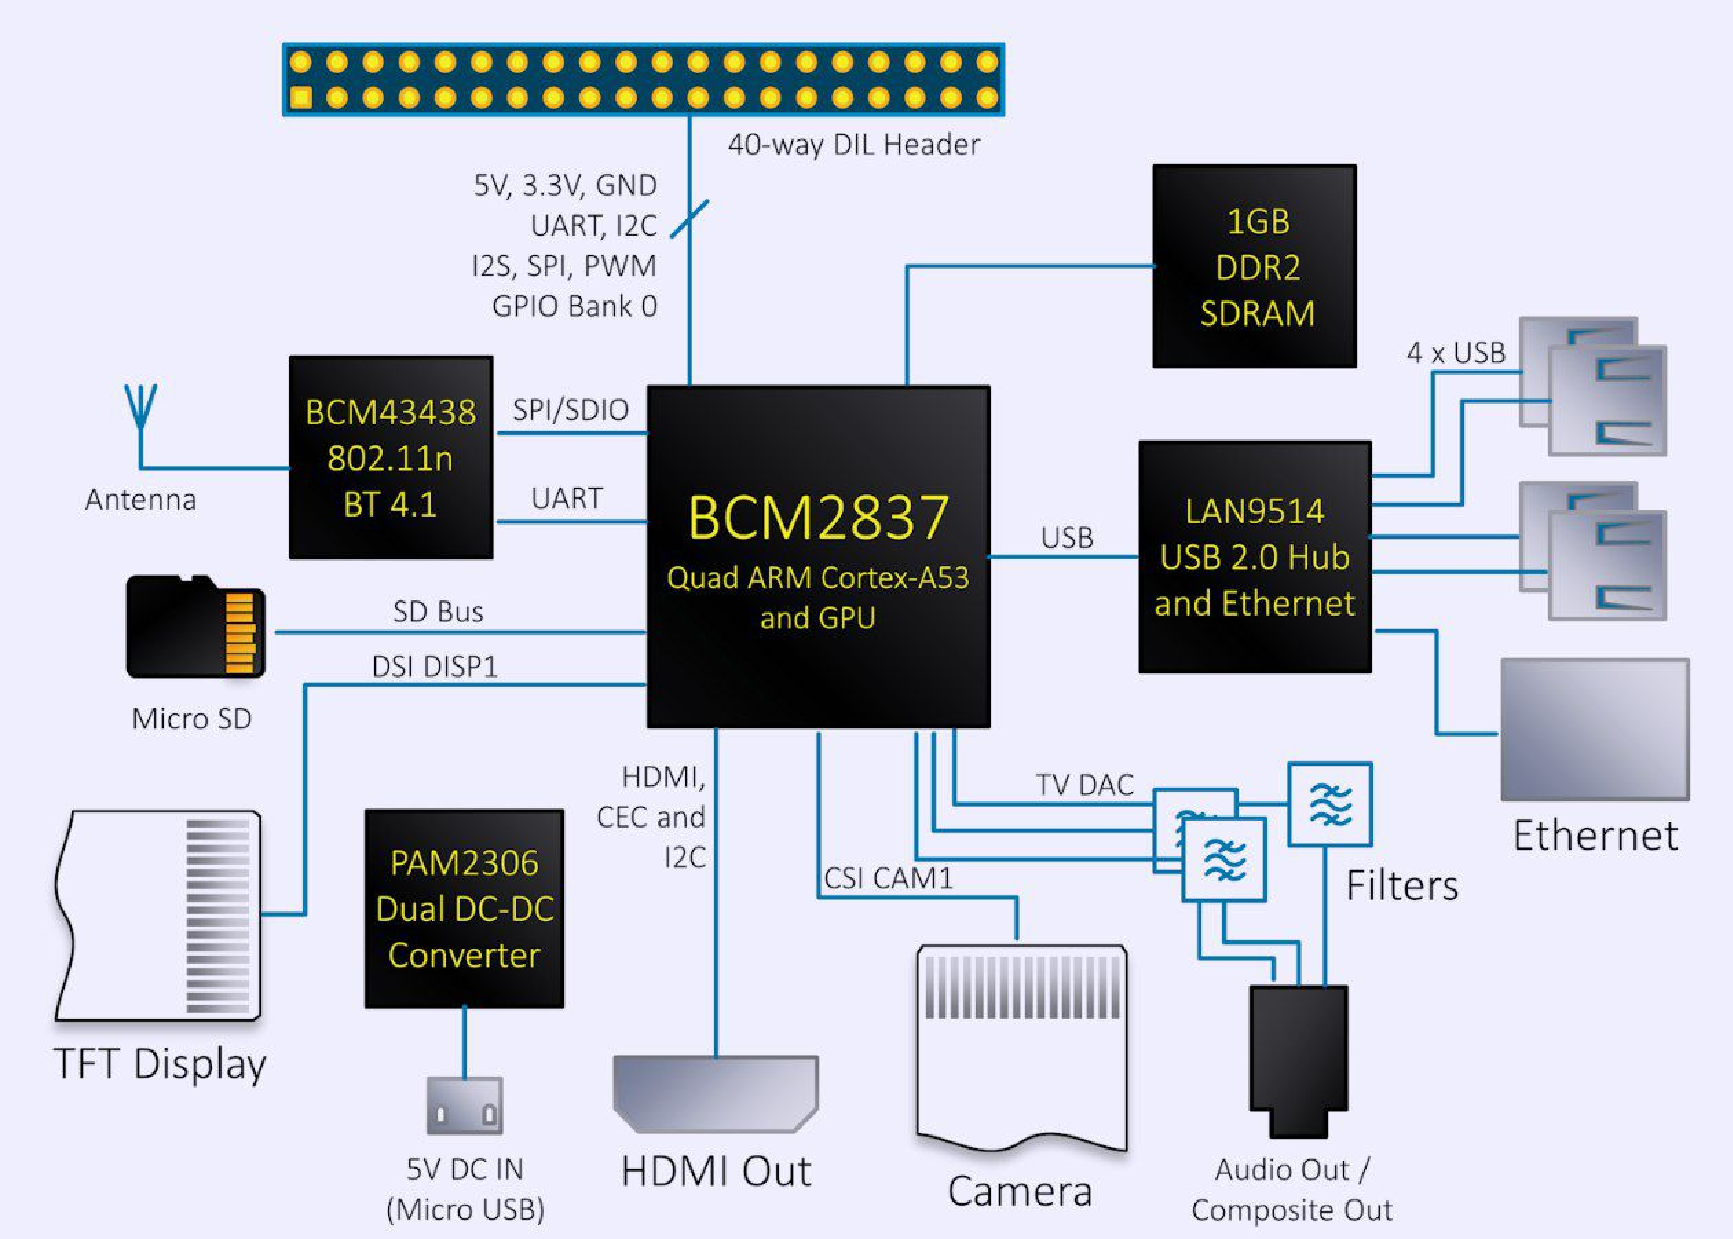
\includegraphics[width=\textwidth]{raspSchema.pdf}
\end{center}
Полную принципиальную схему можно найти \href{https://datasheets.raspberrypi.com/rpi2/raspberry-pi-2-b-reduced-schematics.pdf}{здесь}.

\subsection{Cхема подключений}

Пин №1 подает 3.3 \unit{\volt} на кнопки. Пин №2 подает 5 \unit{\volt} питания на логическое устройство. Моторы питаются из внешнего зарядного устройства.
\begin{center}
  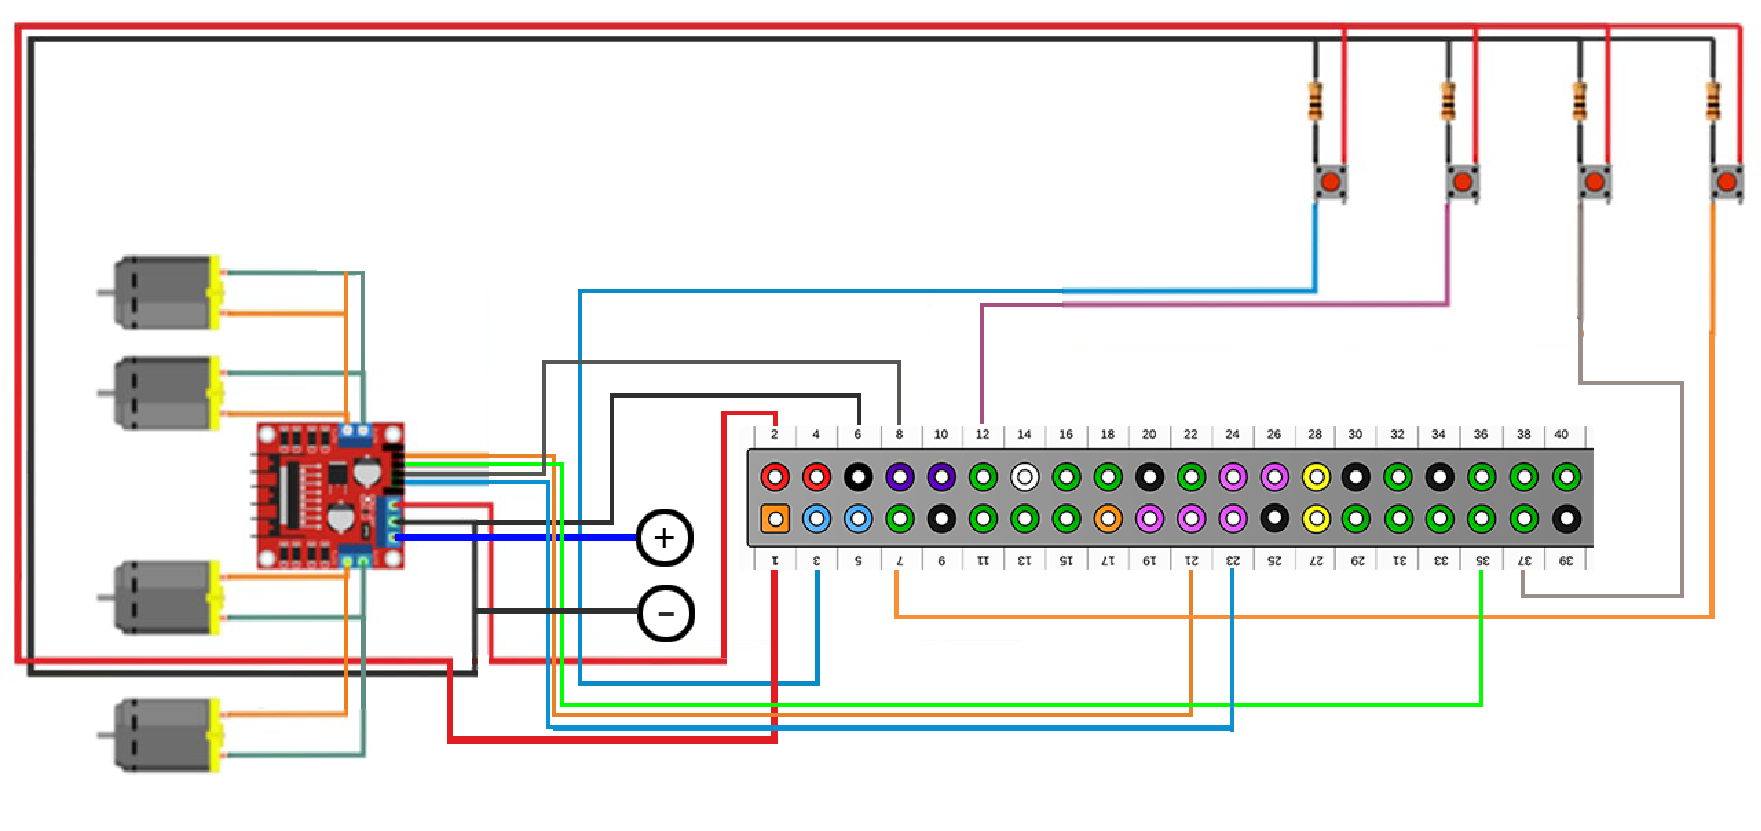
\includegraphics[width=1.0\textwidth]{energy_first.pdf}
\end{center}
\begin{center}
  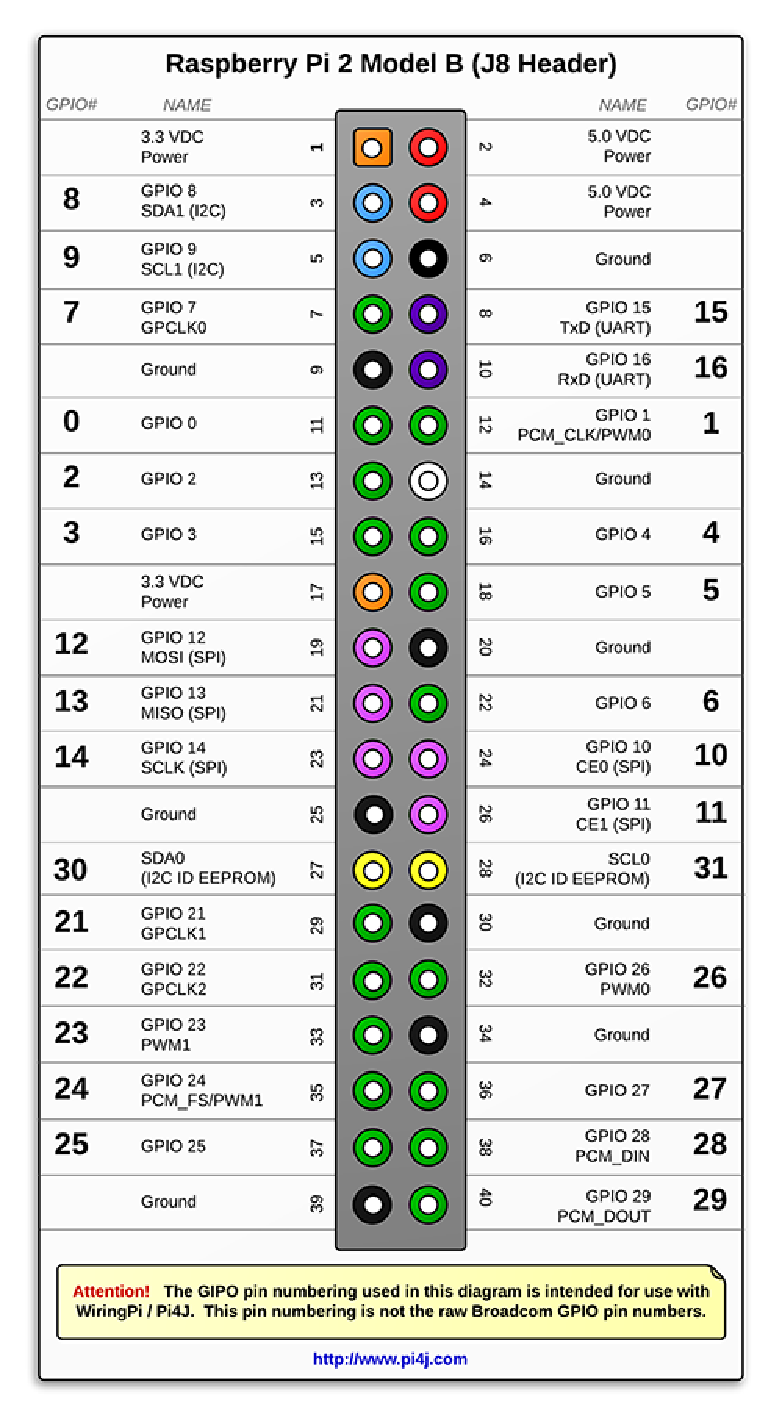
\includegraphics[scale=0.5]{pins.pdf}
\end{center}

Raspberry Pi питает от micro-USB, который подает 5V.
\begin{center}
  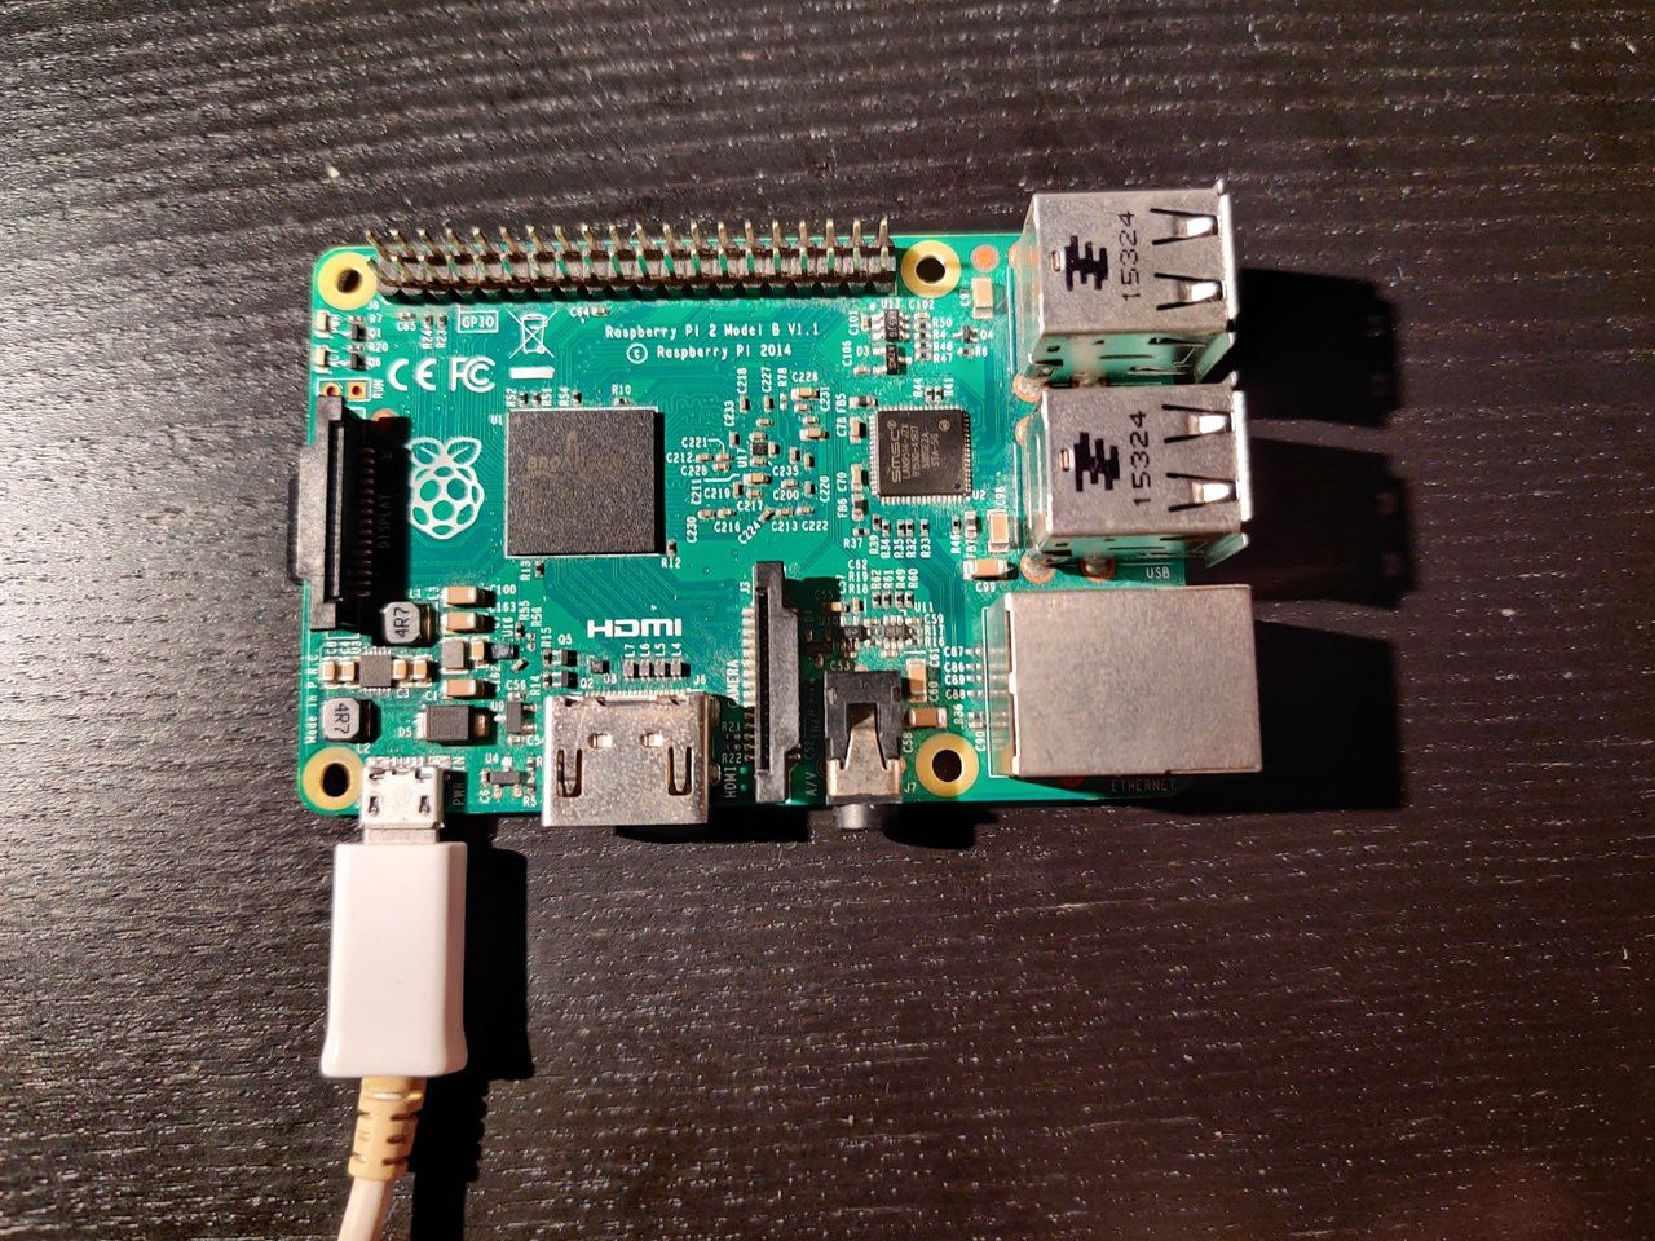
\includegraphics[width=0.8\textwidth]{raspberry.pdf}
\end{center}

\newpage
\section{Rust}
Для написания программы нами был выбран молодой язык программирования Rust. Но почему мы его выбрали?
\begin{description}
  \item[Производительность] Rust невероятно быстр и эффективно использует память:
  без среды выполнения или сборщика мусора он может поддерживать критически важные для
  производительности службы, работать на встроенных устройствах и легко интегрироваться с другими языками.
  \item[Надежность] Богатая система типов и модель владения Rust гарантируют безопасность памяти и потокобезопасность,
  что позволяет устранять многие классы ошибок во время компиляции.
  \item[Удобство] У Rust отличная документация, удобный компилятор с полезными сообщениями об ошибках и первоклассные инструменты
  — интегрированный менеджер пакетов и инструмент сборки, интеллектуальная поддержка нескольких редакторов с автодополнением
   и проверкой типов, автоматический форматировщик и многое другое.
\end{description}

\begin{description}
  \item[Первая Версия] Первый стабильный релиз, Rust 1.0, был анонсирован в мае 2015.
  \item[Владение] Владение — это набор правил, определяющих,
   как программа на Rust управляет памятью. Все программы так 
   или иначе должны использовать память компьютера во время работы.
   В некоторых языках есть сборщики мусора, которые регулярно
   отслеживают неиспользуемую память во время работы программы;
   в других программист должен память явно выделять и освобождать.
   В Rust используется третий подход: управление памятью происходит
   через систему владения с набором правил, которые проверяются
   компилятором. При нарушении любого из правил программа не будет
   скомпилирована.
   \begin{description}
    \item[правило 1] У каждого значения в Rust есть владелец
    \item[правило 2] У значения может быть только один владелец в один момент времени
    \item[правило 3] Когда владелец покидает область видимости, значение удаляется 
   \end{description}
  
  \item[Многопоточность] Безопасное и эффективное управление многопоточным
   программированием — ещё одна из основных целей Rust. Поэтому он обеспечивает
    решение с наилучшей производительностью в любой конкретной ситуации и будут
     иметь меньше абстракций по сравнению с аппаратным обеспечением. Поэтому
      Rust предлагает множество инструментов для моделирования проблем любым
       способом, который подходит для вашей ситуации и требований.
    \begin{description}
    \item[способ 1] потоки для одновременного запуска нескольких фрагментов кода
    \item[способ 2] передачи сообщений, где каналы передают сообщения между потоками
    \item[способ 3] Многопоточность для совместно используемого состояния,
     когда несколько потоков имеют доступ к некоторому фрагменту данных
    \end{description}


\end{description}





\newpage

\section{Реализация на языке Python}
В рамках дополнительного задания нужно было реализовать программу c тем же функционалом на языке Python.
\newpage

\section{Программное обеспечение}
\subsection{Используемые инструменты}
\begin{enumerate}
  \item \href{https://www.rust-lang.org/}{Rust} - 1.65.0 - Язык программирования
  \item \href{https://github.com/golemparts/rppal}{rppal} - 0.14.0 - Raspberry Pi Peripheral Access Library. Предоставляет
  доступ к GPIO у Raspberry Pi.
  \item \href{https://www.python.org/}{Python} -3.10.1 - Язык программирования
  \item \href{https://sourceforge.net/projects/raspberry-gpio-python/}{Rpi.GPIO} - 0.7.0 - Raspberry Pi GPIO. Предоставляет доступ к GPIO у Raspberry Pi.
\end{enumerate}

\subsection{Код программы на Rust}

% \inputminted{rust}{code/main.rs}

% \inputminted{rust}{code/input.rs}

% \inputminted{rust}{code/engine.rs}

% \subsection{Код программы на Python}

% \inputminted{python}{code/main.py}

% \inputminted{python}{code/input.py}

% \inputminted{python}{code/engine.py}

\end{document}